% Generated by documents/paper/figures/make_rq_appendix.py from the rq00_gate_and_curves README; do not edit.
\clearpage
\section{The above-chance gate}
\label{app:rq00_gate_and_curves}

\paragraph{Question.} Which benchmarks clear chance at which size of the ladder, and which separate the language settings most?

\paragraph{Setup.} Seed-1904 runs of every language setting, ladder and data build, 90M--1.7B. A run clears chance on a task when the one-sided 95\% Wilson lower bound of its accuracy over the task's items exceeds the chance level; a (task, size) cell is above chance when at least half of the size's runs that train the task's language clear it. Tasks without a chance level (bits per byte) are not gated.

\paragraph{Key finding.} \textbf{The gate removes most of the evaluation somewhere on the ladder.} On the 841 trained tasks, 312 (37 \%) are above chance at 90M and 489 (58 \%) at 1.7B; 550 (65 \%) are at chance at one size or more, 326 (39 \%) at every size. (Figure~\ref{fig:app_rq00_gate_and_curves}.)

\begin{figure}[h]
\centering
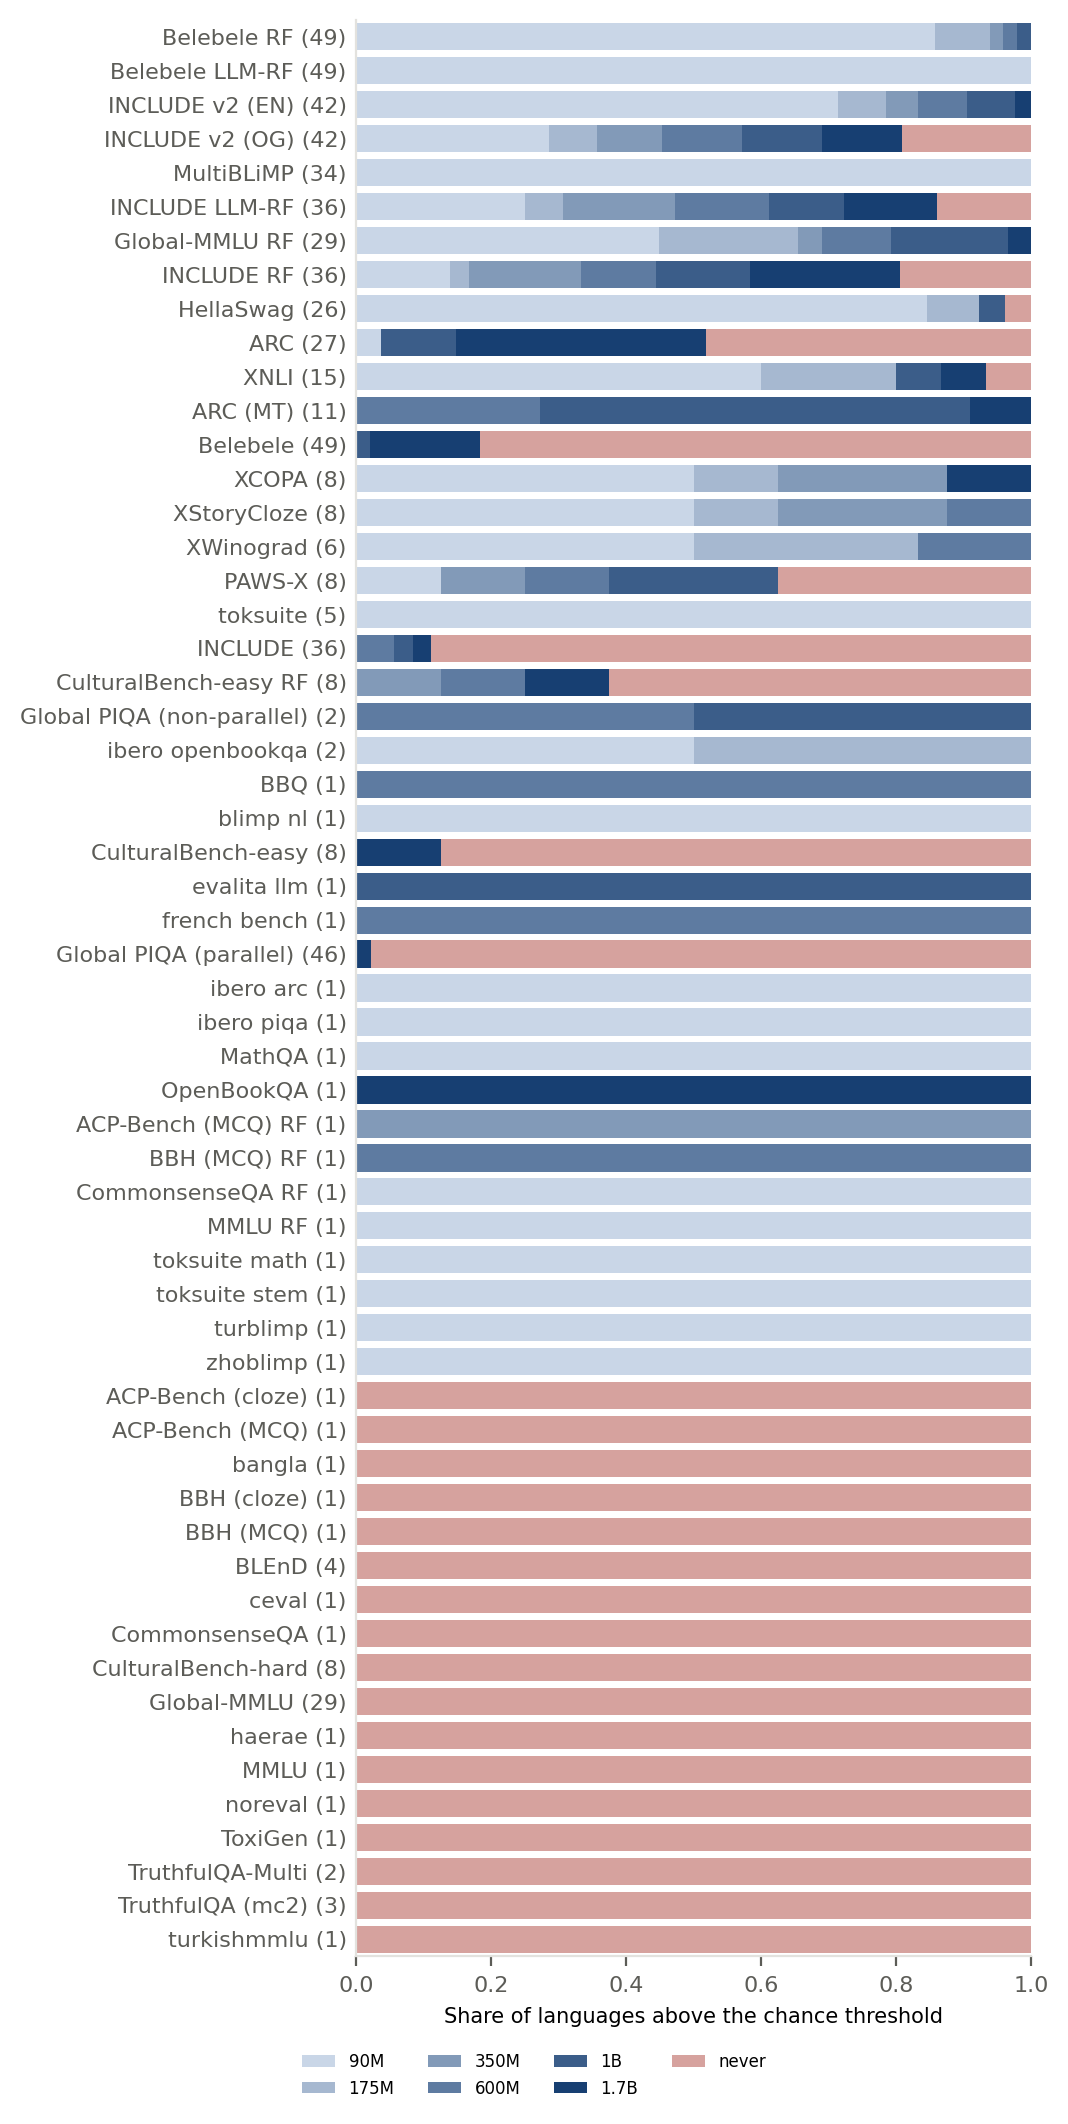
\includegraphics[width=\textwidth]{figures/app_chance_share.png}
% source: src/signal-and-noise/analysis/rq00_gate_and_curves/pretraining/predictivity/first_size_share_paper.png
\caption{Share of each benchmark's language tasks above chance, by the smallest size from which the gate holds.}
\label{fig:app_rq00_gate_and_curves}
\end{figure}
